\documentclass{article}
\usepackage{graphicx} % Required for inserting images

\title{L1 Sounding Rocket 'Dart' - Preliminary Design Review}
\author{Ash E}
\date{May 2023}

\begin{document}

\maketitle

\section{Introduction}

% test

% PARAGRAPH: justification on this project
% why am I persuing this

Hobby rocketry is a fantastic primer on the development of rocket systems, 
including architecture, 
manufacturing concepts, 
basic aerodynamics, 
simple material science 
and kinematics. 
To understand more about sounding rockets 
and to gain a qualification to work on higher power rocket systems, 
the author will develop an L1 sounding rocket as classified by the VRA.

% PARAGRAPH: what is contained in this report?

This report will outline the specification and design 
of an L1-class rocket intended for a certification attempt.

\subsection{Rocket motor classification}

% PARAGRAPH: background on amateur sounding rocketry

'Hobby' or 'amateur' rocketry typically use solid rocket motors (APCP) for propulsion. 
Rocket motors are supplied by approved manufacturers, 
and are classified by their impulse class. 
High-power rockets have certain restrictions on who can manufacture them 
and where they can be flown. 
L1's are the smallest high-power rocket level, 
and can reasonably be constructed 
and certified by individuals with limited experience (Table 1).

% TABLE: sounding rocket classification
% https://nswrocketry.org.au/membership/certifications/
\begin{table}[]
    \centering
    \begin{tabular}{c|c|c}
         Classification & Letter code & Upper impulse range (Ns) \\
         \hline
         Mid-power & G or smaller & 160 \\
         L1 & H,I & 640 \\
         L2 & J,K,L & 5120 \\
         L3 & M,N,O & Above 5120\\
    \end{tabular}
    \caption{VRA/Tripoli motor classification levels}
    \label{tab:my_label}
\end{table}

\subsection{L1 rocket certification}

% PARAGRAPH: what is the nature of L1 sounding rockets
% what components do they usually have, how do they operate

L1 rockets are typically unguided, 
uncontrolled, 
single stage sounding rockets. 
Their recovery system is triggered by a timed explosive charge attached to the motor, 
ejecting a parachute from the top of the rocket body. 
They do not require any electronic systems (unless as a payload).

% PARAGRAPH: L1 certification guidelines
% https://www.tripoli.org/Level1
To perform an L1 certification flight:
\begin{itemize}
    \item The certification flight may occur at any insured launch.
    \item The certifying member (designated Range Safety Officer) must be present 
	and witness the certification flight.
    \item The certifying member must see the rocket ascend stably 
	and descend in a manner controlled by the recovery system.
\end{itemize}

The rocket must be verified to be in a sufficient condition after launch that it could be launched again without repair 
(though the motor needs to be replaced). 
The recovery system must have been deployed successfully, 
the fins and body structure must be undamaged, 
and the rocket must be in one piece (if not staged).

\section{Mission}

% concept of operations
% how do I envision the rocket will operate
% PARAGPRAH: prelaunch procedure

Prior to launch, 
the recovery system (parachute and protective cloth) will be packed into the rocket 
and the motor will be installed into the motor assembly. 
The rocket will undergo a safety review by the designated RSO, 
verifying that there are no obvious flaws with the construction of the rocket 
and verifying that the simulated flight parameters meet the minimum safety criteria. 
The rocket will be slid onto the launch rail, 
and the ignition charges will be fed into the motor from the rear of the rocket.

% PARAGRAPH: launch profile

When approved by the RSO, 
the rocket motor will be ignited and the rocket will launch. 
The rocket will rapidly accelerate 
and ascend unguided to an altitude around 0.7-2 km in the air. 
An ejection charge will be triggered around the peak of the rocket's trajectory, 
deploying the parachute intact. 
The rocket will slowly descend to the ground, 
slowed by the parachute. 
People on the ground will visually track the rocket as it returns to the earth, 
and note down the bearing of it's landing site. 
Once grounded, the rocket will be recovered by ground teams on foot.

\section{Requirements}

% PARAGRAPH: system constraints
% we also specify a particular implementation here based on typical L1 rockets
% to save us time with designing it from scratch and to meet VRA safety guidelines

The rocket system must satisfy the following requirements.

\begin{enumerate}
    \item The rocket shall use an L1-class APCP solid rocket motor, 
	exceeding 5:1 ratio of initial thrust to gross lift-off weight.
    \item The rocket shall be passively fin-guided, 
	with a stability calibre exceeding 1.3 off the launch rod, and below 2.0 overall.
    \item The rocket shall utilise a parachute recovery system, 
	with a decent rate below 9 m/s.
    \item The rocket shall utilise two launch lugs for a 1010 rail profile, 
	with the lower lug positioned at the centre of mass.
\end{enumerate}

\section{Conceptual design}

\subsection{System architecture}

% PARAGRAPH: system components
% and at a high level what implementation we are selecting for each component

Below is a breakdown of the sounding rocket systems:

\begin{description}
    \item [Nose cone] Ogive nose cone, manufactured in PLA using FDM. 
	The cone surfaces were sanded to a smooth finish.
	 There is an attachment point for a shock cord.
    \item [Body tube] ID60x660 mm cardboard body tube. 
	Wall thickness of 2 mm.
    \item [Thrust structure] Consists of a thrust ring at the base of the motor, 
	centring ring at the top of the motor, 
	and the tabs of the fins. 
	Rings and fins consist of 3 mm plywood segments. 
	Motor tube is a ID38x220 mm cardboard tube, 
	with wall thickness of 1 mm. 
    \item [Fins] Trapezoidal fins, 
	made of 3 mm plywood segments.
    \item [Recovery system] Parachute and Nomex package that is ejected through the top of the body tube.
    \item [Launch guides] 1010-rail lugs.
\end{description}

% following sections go into more detail on the design choices made for each component, justification etc

\subsubsection{Nose cone}

% PARAGRAPH: justification on nose cone design, how we will construct it, technical details

The nose cone is selected to be 'ogive' as it is the most efficient shape for subsonic rockets.

\subsubsection{Body tube}

% PARAGRAPH: justification on body tube design, how will we construct it, technical details

The rocket is designed around a medium (60x660 mm) Auspost mailing tube. 
These tubes are designed to be physically robust

\subsubsection{Thrust structure}

% need to update the solidworks model

% Rules:
% the thrust ring should be positioned far enough down the motor tube that it allows the retainer to be epoxied in
% the fin tabs need to be constrained to the rings
% how long is the rocket motor?

% PARAGRAPH: justification on thrust structure design, how we will construct it, technical details

The thrust structure is responible for securing the rocket airframe to the motor. 
It transfers the thrust force into the body tube 
and constrains the motor from exiting the tube.

The motor tube is set to an inner diameter of 38 mm. 
This allows 38 mm or 29 mm motors to be accepted, 
though 29 mm motors will need an adaptor.

\subsubsection{Fins}

% need schematic of the fin shape
% talk about four fin design. it produces more drag but it draws back the CP

% PARAGRAPH: justification on thrust structure design, how we will construct it, technical details

\subsubsection{Recovery system}

% need a diagram of the recovery cord, parachute, where it attaches to the rocket components and how it is connected (tied, through carabaner clips, etc).

% Rules:
% shock cord to be ~2 times the length of the rocket
% design the parachute size to the mass of the rocket

% PARAGRAPH: justification on recovery system design, how we will construct it, technical details

\subsubsection{Launch guides}

% type of rail guides, where they are positioned
% where they are secured to the rocket (i.e. body tube)
% rocket is below 15kg so doesnt need 1515 rails

% PARAGRAPH: justification on launch guides, how we will construct it, technical details

\section{Simulation}

% PARAGRAPH: what is simulation and why do we need it here?
% PARAGRAPH: how will we simulate this

The rocket was modelled in 'OpenRocket,' 
a free rocket simulation software. 
OpenRocket software is good to simulate basic sounding rockets that travel below the speed of sound, 
and can validate several key requirements.

% PARAGRAPH: present results of simulation

Below is the rocket design, using a H135T motor. 
The aerodynamic profile and recovery system are included, 
though some minor details (such as launch lugs) were not modelled.

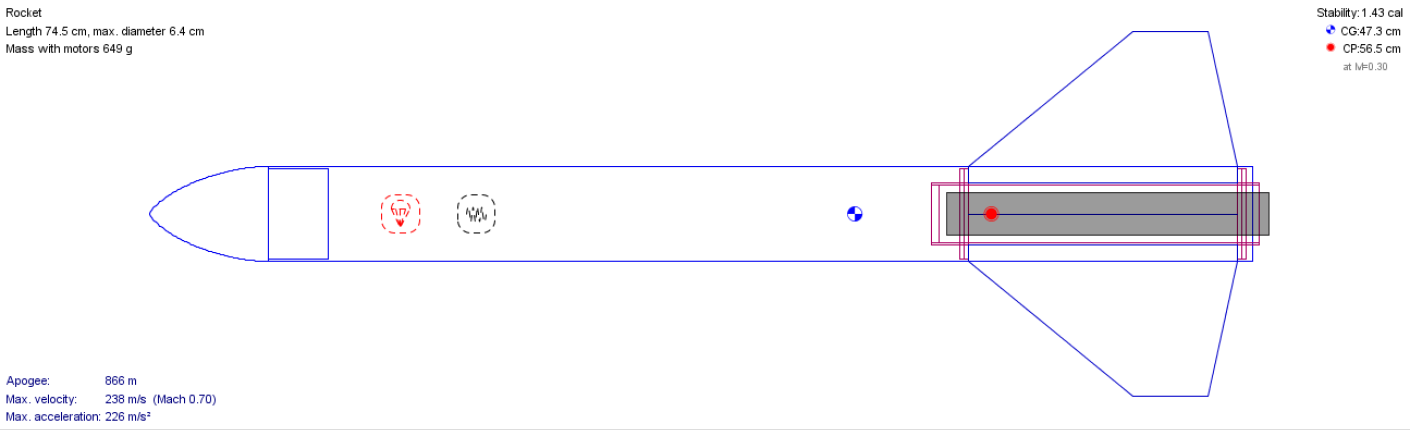
\includegraphics[width=\textwidth]{images/rocket model 7-5-23.png}

To understand the effect that different motors have on the flight profile of the rocket, 
three H-class motors were selected and simulated. 
This will help inform the optimisation of the rocket profile once the specific motor configuration is selected.

% TODO: flesh out this section

\subsection{System performance metrics}

% against requirements:
% Thrust to weight
% - i've only weighed the nose cone and body tube
% stability calibre over time
% final descent rate

\subsection{Flight performance}

% altitude, flight, acceleration
% - need to consider the velocity and stability of the rocket at this point. i'm a little concerned about the rocket tumbling if the SC dips too low. however, a small angle in the launch rod or a small wind should give the rocket enough velocity to make it through it's apogee stable
% - mention ejection charge!!!

\end{document}
